\chapter{Method}
Given the aim of this project, we now present the methodology. We then present the three cases that are of attention in this project.


\section{Research Methodology}
The aim of this project is to develop a method of analysis that identifies hidden relations in a document database. To perform this, an inductive research design has been taken. Starting off by studying a few specific cases, the expectation is to find some pattern leading to a broader generalization. From there, tentative hypothesis will be formulated which later will be tested and hopefully conveyed into a final conclusion.

\section{Research Design}
% To identify relevant cases, interviews will be held
Taking the inductive approach, the first thing to do is to identify important and representative cases. Thus, the research starts with interviewing analysts at Recorded Future with the result being a list of questions related to their data that are hard to answer based on the existing database and software. This will give us information about what kind of relations that are interesting to look at from a security analyst perspective.

\section{Validation} 
The final step of the study concerns validation. The developed method must be validated to tell whether it is performing well or not. The validation will be performed on a sample of chosen cases, for which the answer is known. The answer could be figured out by for instance perform extensive analysis in multiple steps with the existing database and software.

\section{Introduction to the Data Set \label{dataset}}
The data of Recorded Future is comprised of entities, e.g. a country, a person or a company. They are in turn often a component in an ontology, such as Stockholm being part of Sweden. Another central concept is references, often connecting two entities. References are a report or text fragment related to a specific event. Furthermore, there is metadata that can be different sorts of data related to entities and events, such as a time interval or type of entity or event.

The data is fetched by queries using Recorded Future's API. The output is a file in JSON format. As previously mentioned, the database contains a lot of information. Thus, it is essential that only a subset of the data is fetched. This leads to the issue of querying the right information and only the right information. To be able to answer a question, we want to have all the necessary information at hand without dealing with too much information. This is based on two reasons; querying information takes time and the more data the more complexity arises.

One difficulty with the data is that some parts are implicit. Since Recorded Future are dealing with natural language processing there are cases when all the information about an event is not available. For instance, if someone on the Internet is writing about a cyber attack they might mention an attacker and malware without specifying the target, hence creating implicit data. 

Another important aspect is that the data does not reflect the real world but what users on Internet find interesting to report. Hence, on one hand there might be some information missing, while there on the other hand may be much data on one single event due to various reasons. An example of the latter case is if Donald Trump's personal computer would be hacked by a hacker representing Anonymous. Due to the popularity of both Trump and Anonymous, it is likely that many people writes about this all over the Internet resulting in many references about this specific happening. Thus, the question arises whether there have been multiple attacks or only one. Studying the time of the reports may reveal a lot of information enabling to answer the previous question however there might be cases where there is periodic interest to report about a certain happening. The latter is far more ambiguous.

\section{Extracting Relations From a Document Database}
% Motivate the need to use a graph database
To reduce the time spent on extracting the right kind of data, a graph database has been created

% Introduction to Neo4j
Neo4j is a graph database management system that has a query language Cypher and let the user interact with 

% How is the extraction and import to Neo4j performed?
In many cases, document databases has a nested structure. Thus, it is necessary to flatten out the data

\section{Graph Representation}
Data modeling with graphs are highly domain dependent and highly dependent on what type of question one is trying to answer. Thus, according to \citet{robinson2013}, the following approach should be taken:
\begin{itemize}
    \item Describe the goals that motivate the model.
    \item Rewrite the goals as questions to ask the domain.
    \item Identify the entities and the relationships that appear in these questions. 
    \item Translate the entities and relationships into Cypher path expressions.
    \item Express the questions we want to ask of our domain as graph patterns using path expressions similar to the ones we used to model the domain. 
\end{itemize}

\section{Revealing Hidden Relations}

% Motivate the choice of algorithms
The usefulness of the algorithms and measures highly depends on the task \cite{fouss2016algorithms}. It is therefore necessary to perform empirical tests and validate the relevance. 

Algorithms for analysis has been chosen to be as simple as possible yet give a satisfactory result. 


\section{Introduction to the cases}
Below we present the three cases which has been studied. They were chosen to give a representative view of the questions one might want to address using a graph representation. Also, the cases have been chosen to show the width of use cases that a graph representation could cover.

\subsection{Gh0st RAT Controllers}
Gh0st RAT (Remote Access Terminal) is a Trojan horse used to hack and take control of computers in real-time. The malware has been used to hack some of the most sensitive computers in the world.

Our data consists of NetFlow data related to a number of IP addresses that have been identified as Ghost RAT controllers. The data is annotated such that known RAT controllers have been annotated with the label \textit{Ghost}. There is also information of the IP traffic such that it is known which IP address that has communicated with whom. Thus, in this case our graph model consists of IP addresses as nodes with the relations ``COMMUNICATED'' between them if they have communicated. The graph is modelled as an undirected graph, since the RAT controller-slave communication could have been initiated in any direction.

We have two similar data sets. The first set is based on 21831 NetFlow records collected during the first months of 2017. In total, the data consist of 3566 IP addresses where 204 of them have been identified as RAT controllers using packet inspection of responses from RAT controllers. A topographic view of the network can be seen in figure \ref{ip1}.

\begin{figure}[h!]
    \centering
    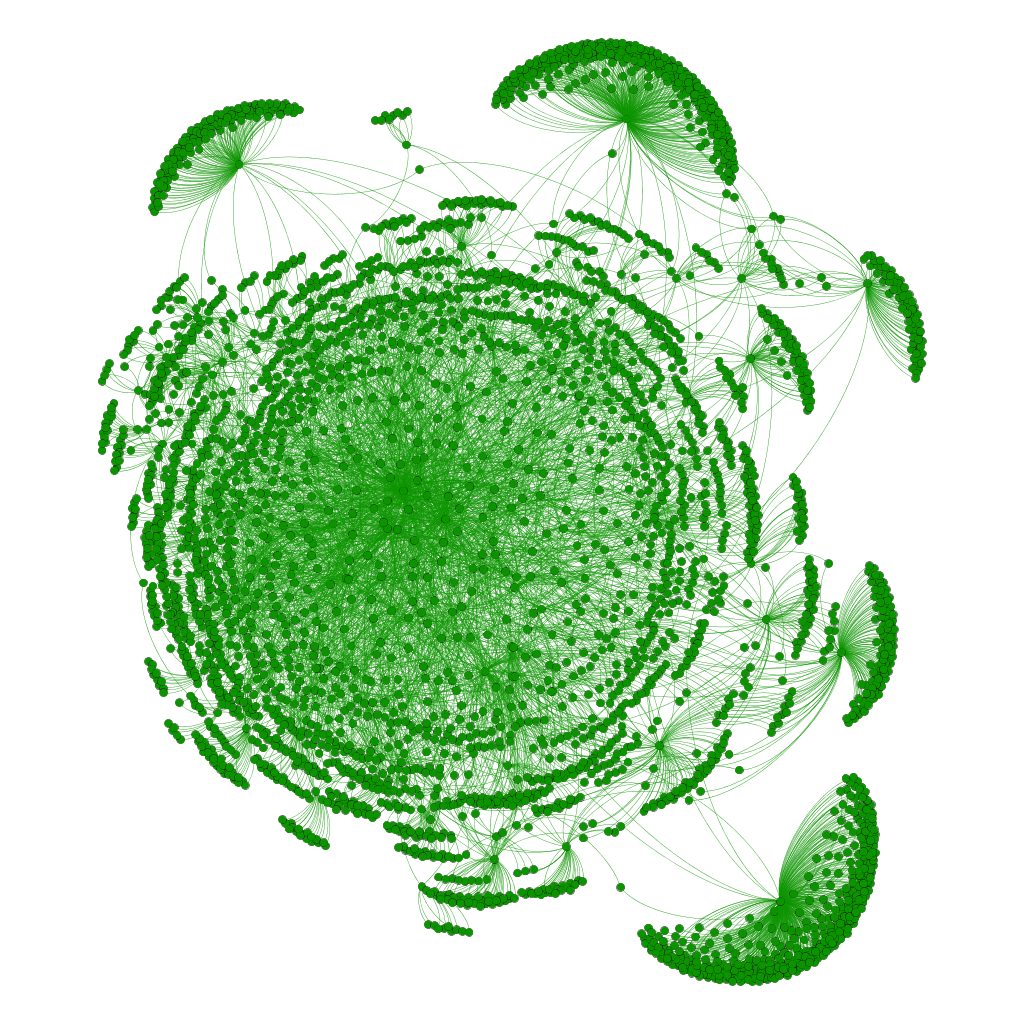
\includegraphics[width=0.5\textwidth]{GhostRATs.png}
    \caption{Graph of IP addresses, consisting of 3566 nodes with 204 known RAT controllers. The graph is visualized using Gephi.}
    \label{ip1}
\end{figure}

The second data set consists of 103202 NetFlow records collected during December 2016 to Mars 2017. This data set includes 10091 IP addresses but is far more sparse with \textit{Ghost}s, containing only 32 identified RAT controllers. 

In this case, we have aimed at classifying the IP addresses, given the notion of only a few RAT controllers. As a consequence, we also aimed at identifying IP addresses that are falsely annotated as \textit{Non-ghost}s. Moreover, this study involves a comparison between the seven different measures of structural equivalence. 

The classification has been performed by applying different similarity measures to the network. The applied similarity measures are the Dice coefficient, the Jaccard index, the cosine coefficient, the hub-promoting index and the hub-depressing index. Thess are all measures of structural equivalence and reflect the similarity based on the local structure, i.e. only the overlap of nearest neighbors.

Furthermore, the Local Path index and the Katz index were studied. Instead of simply studying the information of the nearest neighbors, they also account for more information about the topology. However, both of these indices have a discounting factor $\alpha$ that had to be chosen. For the Local Path index, $\alpha$ was chosen to 0.1. For the Katz index, $\alpha$ was chosen to 0.2. %However, the two involves the parameter $\alpha$ that should be properly chosen. To chose it, a fraction of the dataset (20 \%) was used to chose the best value of the parameter. 

The similarity was calculated for all nodes, given a small portion (1-5) of known Gh0st RAT controllers, henceforth referred to as reference nodes. Thus, the similarities for one node, in relation to the others, were simply taken as the sum. To classify the node, a threshold was then applied. If the similarity value exceeded the threshold, the node was classified as a RAT controller, i.e. a \textit{Ghost}.

Once the classification was performed, the classifier using different similarity measures was evaluated. The evaluation was based on the AUC of the precision recall curve and the F$_1$ score. AUC can be interpreted as a value of robustness of the similarity measure while F$_1$ represents the accuracy.

\subsection{Classification of malicious IP addresses}
In this case, we have 102056 IP addresses from the Recorded Future database. In the graph, the IP addresses are represented as nodes with relations referred to as ``RELATED TO'' in between. The reason the relations have that specific label is because of the nature in which we do not know any more specific details about their co-occurrence. Furthermore, in the graph there are nodes related to malware, attack vectors and cyber vulnerabilities. These has served as additional information which has been used as information about the neighboring IP addresses.

Recorded Future classifies the IP addresses based on roughly 40 rules. There are 5 different classes
\begin{enumerate}
    \item None
    \item Unusual
    \item Suspicious
    \item Malicious
    \item Very Malicious
\end{enumerate}

The histogram of the classifications of the dataset is shown in \figref{hist}. We find the data to have an exponential distribution function, being extremely skewed to the left. Class 1 includes 60 \% of the data, class 2 33 \%, class 3 4 \%, class 4 2.5 \% and class 5 0.5 \%. 

\begin{figure}[h!]
    \centering
    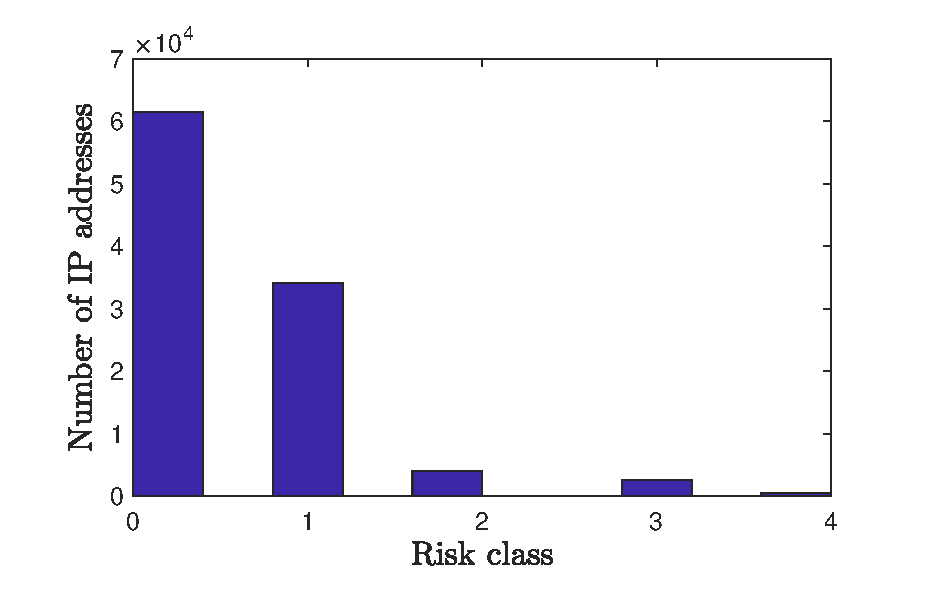
\includegraphics[width=0.6\textwidth]{histData.eps}
    \caption{Histogram of the data classifications.}
    \label{hist}
\end{figure}

This case treats the study whether a graph approach with far less information might be enough to reconstruct Recorded Future's rule based classification. Removing any of their enriched data, we have simply used data found in the original reference. Thus, as a consequence, the following bold question is asked \textit{Is there a way of reconstructing Recorded Future's rule based classifier using a graph representation?} 

To classify the nodes, we have implemented a feature based node classifier. Using features based on topological information, predictions about their criticality was performed.

% Feature extraction
The term feature extraction refers to methods used for constructing node variables from the structure of the graph. These features were then used a input parameters for the classifier. Thus, the performance is highly dependent on the choice of features. In our case, the following features were used
\begin{itemize}
    \item PageRank based on the topology of IP addresses.
    \item Degree based on an undirected graph including only the IP addresses.
    \item Total number of hits in Recorded Future's data base.
    \item Number of unique malwares related to the nearest neighbors.
    \item Number of unique cyber vulnerabilities related to the nearest neighbors.
    \item Number of unique attack vectors related to the nearest neighbors.
\end{itemize}

The features can be divided into two categories. The first includes the PageRank and degree, only including the topology of the graph including only the IP addresses. The second category includes more information from Recorded Future's database, such as the number of hits, co-occurrences with malwares and so on. To study the impact of the different categories of features, classifications were performed including all of the features, only the topology features and finally the features including information regarding the number of hits, malwares, cyber vulnerabilities and attack vectors.

% Choice of classifier
Five different classifiers were briefly evaluated by studying the accuracy of prediction for only two variables at a time. Only two variables were chosen in order to be able to view the results in a 2D chart. The different classifiers were Random Forest, Quadratic Discriminant Analysis, Logistic Regression, Nearest Neighbors and SVM using a radial basis kernel. Predicting almost equally good, the SVM was slightly better than Nearest Neighbors. Hence the SVM was chosen. The fact that it was easily extended to a multi-class classifier was also an advantage. In addition, many researchers have used SVM for feature classification and found good results \citep{campbell2011}.

The SVM takes a matrix of features as input. As mentioned in \secref{scale}, it is preferable to rescale the feature vectors to avoid that some features are dominated by others. The rescaling was performed for each and every feature, in the range $[0,1]$, keeping the interrelation between elements in the feature vector. This is in accordance with the recommendation of \citet{Hsu10apractical}.

After choosing the SVM classifier with radial basis function, the parameters $C$ and $\gamma$ had to properly be chosen. In order to do so, a grid search was performed. Various pairs of $C$ and $\gamma$ was tried and evaluated based on cross-validational accuracy of 10 \% of the data. This was to avoid the pitfall of overfitting to the only dataset available. Once again in accordance with the recommendation of \citet{Hsu10apractical}, an exponentially growing sequence of parameters were studied where $C\in\{10^{-2},10^{-1},10^{0},...,10^{3}\}$ and $\gamma\in\{10^{-3},10^{-2},...,10^{2}\}$. The evaluation of the classifier was based on the accuracy, referring the the fraction of correct predictions. The set of parameters were chosen by maximizing the accuracy while making sure the predictions included all five classes. Since three different sub-cases were studies, each including a different set of features, the grid search was performed for each individual case. 

% Cross-validation including split into training and test set
After implementing the classifier, it needed to be validated. Because of the regularization parameter $C$, SVM does not imply any big risk of overfitting. Thus, a k-fold cross-validation was applied. We used 10 folds and 20 repetitions, in order to get a good statistical foundation.

Because of the skewness of the dataset, a pseudorandom classifier, based on a uniform distribution, was also implemented.  The results from it was then used in order to evaluate the SVM results. 

\subsection{Cyber Attacks}\label{cyberattacks}
Recorded Future's database contain entities that represents an event called cyberattack. The cyberattack entity is based on information found on the open internet as well as the dark/deep web. The entity may contain information such as the time when the attack is believed to have taken place, the author of the source of information, possible attackers and target as well as vulnerabilities and methods used to mention a few.

The whole set of cyberattack events is quite large. To predict future cyber attacks by the method of link prediction bipartite graphs described in \secref{sec:plp} we used only a subset of the cyber attack entities containing only the entities with a mention of an attacker and a target. The size of the subset containing all such references was 1435073. The number of cyber attacks that was indexed as taken place last month was 36297 which indicates how fast the subset we are using for analysis is growing.

The cyber attacks in the data set was represented in bipartite graph with the two adjacent sets being attackers and targets. It is worth mentioning that there are several cases where an entity appears as an attacker in one cyber attack and later as a target in another cyber attack. This goes against the definition of the bipartite graph. The solution was to create two different vertices representing in one case an attacker and in the other a target for such entities. The number of references for each attacker-target pair was used as the weight of the edge between the attacker and the target of the attack in the graph.

The running time of the PLP-algorithm by \citet{plp}, described in section \secref{sec:plp} is O(m) with m being the size of the smallest of the two adjacent sets of nodes in the bipartite graph. The subset we used is containing XX unique attackers and YY unique targets. And hence the running time will be O(a) where a is the number of attackers.

Even if PLP is quite efficient the running time could be reduced even further if link prediction could be made with good accuracy using only the most recent cyber attacks. Therefore we we investigated how the number of prediction and the precision was affected by different of length of time periods used for prediction. We were also interested in finding out what can could be said about when a predicted attack will take place and therefore we also varied the length of the time period used for testing the predictions.

To get good statistical values we repeated each experiment 10 times by randomly picking a start date for the prediction data set. We then computed the average values together with the standard deviations.

To evaluate how well PLP was able to predict future cyber attacks we primarily used two values. 
\paragraph{AUC}\label{plp:auc}
We wanted to find out how often the predictive index was higher for attacks that existed in the test set than for predictive indexes for attacks that was not in the test set. We therefore measured the AUC as
$$
  AUC = \frac{A+0.5C}{n},
$$
where A is the number of times where the existing attacks had a higher index, C is the number of times the index was the same and $n$ is the number of comparisons. We see that if the existing attacks has a higher index in all comparisons the precision is 1, if all compared index is equal the precision is 0.5 and if the index was higher for all non-existing attacks the precision is 0.

\paragraph{Prediction Rate}\label{plp:predict_rate}
Since PLP only gives a predictive index for the candidate node pairs it is reasonable to evaluate how many of the attacks in the test set that was given prediction index. We computed the prediction rate simply as
$$
  \frac{p}{m},
$$
where $p$ is the number of attacks in the test set that was given an index by PLP and $m$ is the number of attacks with unique pairs of attackers and targets.

The algorithm is naturally limited by that it is not able to predict attacks where the attack-target pair exist in a attack already in the prediction set. The algorithm is not able to predict attacks involving attackers or targets not in existence in the prediction set. Based on this it is interesting to see how many of the attacks in the test set are attacks that consist of a attacker-target pair not already in the prediction set but with each of the attacker and target individually in the prediction set.



\newpage 
